\section{Methods}

The central aim of the OPQ Project is to provide a scalable source of actionable power quality data about electrical grids, particularly those with high levels of distributed, intermittent power generation.

Our research methodology consists of three (potentially interleaved) phases. First, we specify, design, and implement novel hardware and software for collecting, transmitting, and analyzing four essential measures of power quality data: voltage, frequency, THD, and transients. Second, we verify that our implementation matches our specifications through laboratory experiments.  Third, we validate our implementation by testing a variety of hypotheses through a real-world deployment. In this paper, we report on results from a pilot deployment at the University of Hawaii over the course of three months.

Our central hypothesis is that we can accomplish this through the design and implementation of a low-cost sensor network for power quality using custom power quality monitors with real-time, two-way communication to a set of cloud-based services.

We will test this central hypothesis through six subhypotheses: (1) OPQ provides valid and reliable collection of power quality data (Section \ref{hyp:01}), (2) OPQ's triggering system provides advantages with respect to bandwidth and computation (Section \ref{hyp:02}, (3) OPQ enables subthreshold event detection based upon temporal locality (Section \ref{sec:subthreshold-events}), (4) The OPQ information architecture provides a means to produce actionable insights (Section \ref{hyp:04}), (5) the OPQ information architecture provides predictable upper bounds on storage resources (Section \ref{hyp:05}), and (6) OPQ provides useful adaptive optimization capabilites (Section \ref{sec:adaptive-optimization}).

The remainder of this section presents the overall architecture of OPQ, along with details on the design and implementation of each of the principal architectural components. We will also discuss our verification activities for each component. Our validation and hypothesis testing activities will be described in Section \ref{sec:pilot-study}.

\subsection{OPQ Architecture}

The OPQ system architecture consists of four major open source hardware and software components that provide end-to-end support for the capture, triggering, analysis, and reporting of consumer level local and global PQ events.  OPQ Box is a hardware device that detects the electrical waveform from a standard residential outlet and communicates both low and high fidelity representations of the waveform to other OPQ system components either at predefined intervals or upon request. OPQ Makai monitors incoming low fidelity data from OPQ Boxes, requests high fidelity data when necessary, and stores the results in a MongoDB database. OPQ Mauka analyzes low level data and analyzes it to produce higher-level representations according to the information architecture described below, and can tell OPQ Makai to request high fidelity data from one or more OPQ Boxes to facilitate analysis. OPQ View is a browser-based visualization platform for displaying the results for data capture and analysis.

\begin{figure}
\center 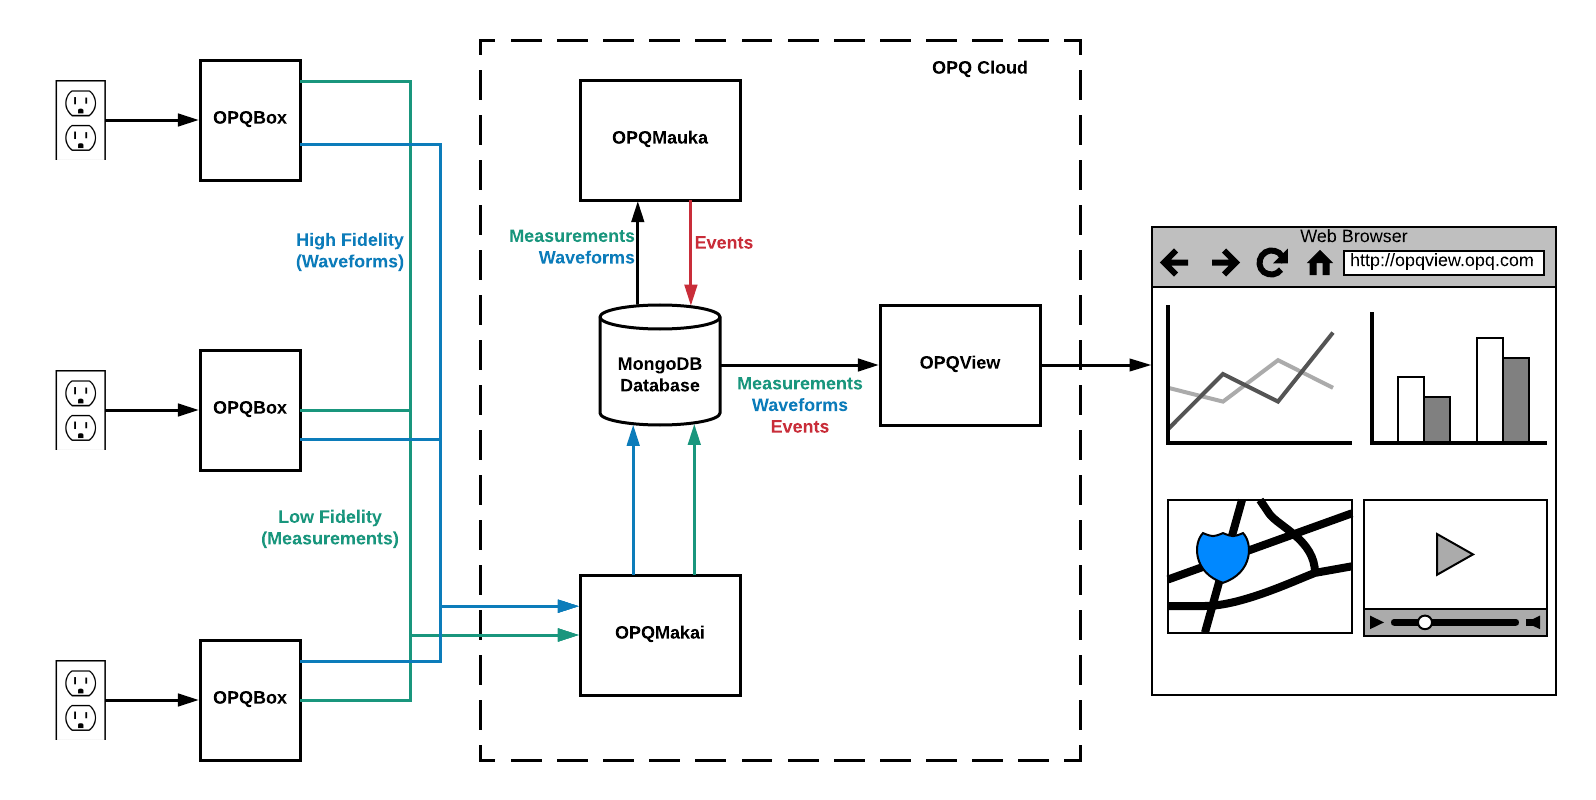
\includegraphics[width=5in]{images/architecture/system-diagram.png}
\caption{High level system architecture of an OPQ Sensor Network}
\label{fig:architecture}
\end{figure}

Figure \ref{fig:architecture} illustrates how these components work together to take information from wall outlets (on the left side) to the display of analyses in a browser (on the right hand side).  First, OPQ Boxes analyze power from wall outlets, and send low fidelity measurements to OPQ Makai. OPQ Makai analyzes low fidelity measurements, and requests high fidelity waveforms when desirable. Both measurements and waveforms are saved in a MongoDB database. OPQ Mauka analyzes low and high fidelity data, and creates "events" to represent anomalies. OPQ View notifies users of events and allows them to drill down into low and high fidelity data.

OPQ Makai, OPQ Mauka, and OPQ View are all cloud-based software services that collectively form a single "instance" with respect to data transmission, storage, analysis, and visualization. We refer to this collection of software-side components as OPQ Cloud. Every OPQ Box connects to a single instance of an OPQ Cloud. It is possible to have multiple OPQ Cloud instances. For example, a company might install an OPQ Cloud instance behind their firewall along with OPQ Boxes to provide a private mechanism for collecting and analyzing power quality data.

\subsection{OPQ Box}
\label{sec:opq-box}

OPQ Box is a hardware device designed to provide inexpensive, extensible and accurate residential power quality measurements.
A block diagram of OPQ Box is shown in Figure~\ref{fig:opq:1:1}.
A complete device is shown in Figure~\ref{fig:opq:1:2}.

\begin{figure}[ht]
	\centering
	\begin{subfigure}{.5\textwidth}
	  \centering
	  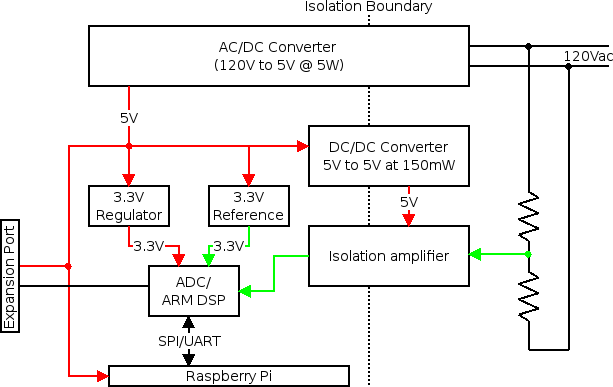
\includegraphics[width=0.9\linewidth]{images/opq-box/opqbox_diagram.png}
	  \caption{OPQ Box Block Diagram.
	  The power path is in red, signal path is in green and the digital IO is in black.}
	  \label{fig:opq:1:1}
	\end{subfigure}%
	\begin{subfigure}{.5\textwidth}
	  \centering
	  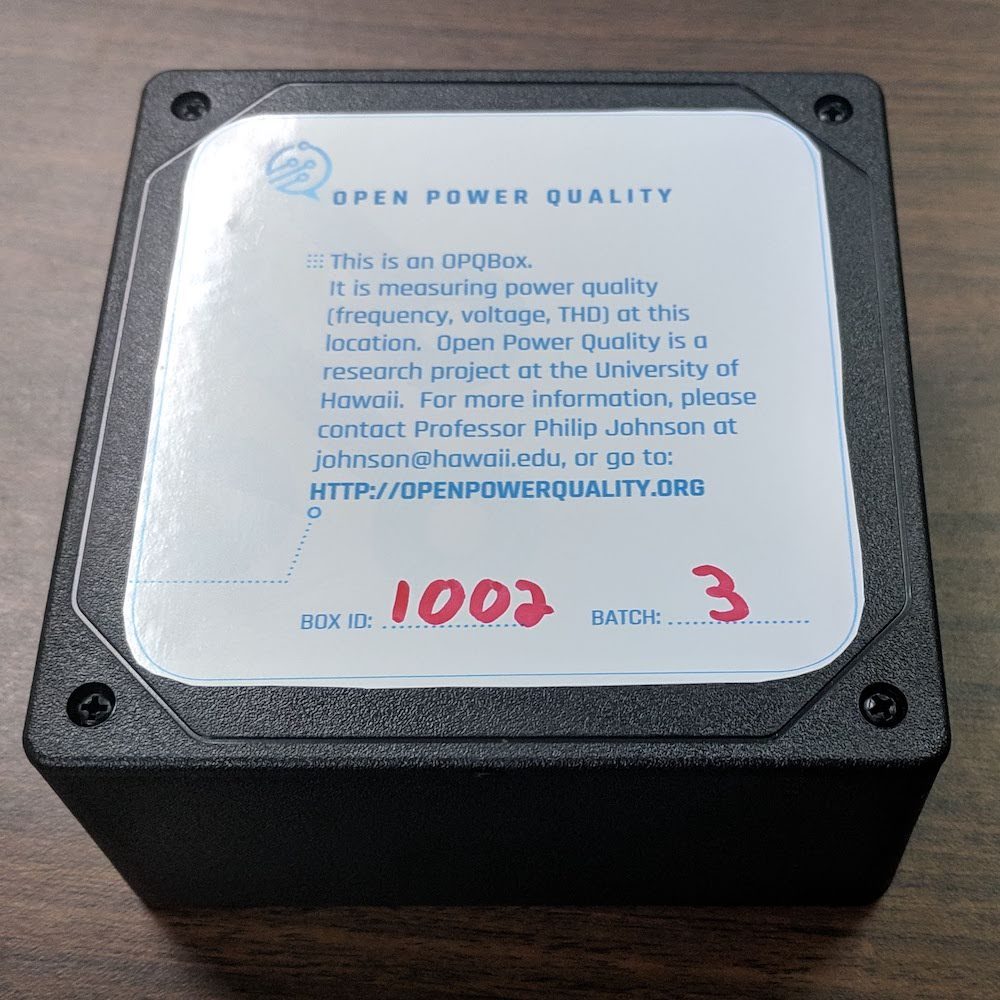
\includegraphics[width=0.7\linewidth]{images/opq-box/opqbox_photo.jpg}
	  \caption{OPQ Box in an ABS plastic enclosure.}
	  \label{fig:opq:1:2}
	\end{subfigure}
	\caption{(a) OPQ Box block diagram and (b) production OPQ Box ready for deployment}
	\label{fig:opq:2}
\end{figure}

\subsubsection{Hardware}\label{subsec:hardware}

The power system of the OPQ Box electrically isolates most of the device from the AC mains power.
An isolated AC-DC converter generates $5V_{dc}$ from the mains $120V_{ac}$.
5V is used to power the Raspberry Pi, the equipment connected to the expansion port, the 3.3V regulators and voltage reference, and an isolated DC/DC converter.
3.3V is used to power the isolated end of the isolation amplifier as well as the STM32F3 analog to digital converter/digital signal processor (ADC/DSP).
The hot side of the isolation amplifier is powered from the isolated DC/DC converter.
This allows OPQ Box to function with a battery attached to the expansion port, so that it may retain data and continue to operate during a power outage.

\begin{figure}[ht]
  \begin{center}
  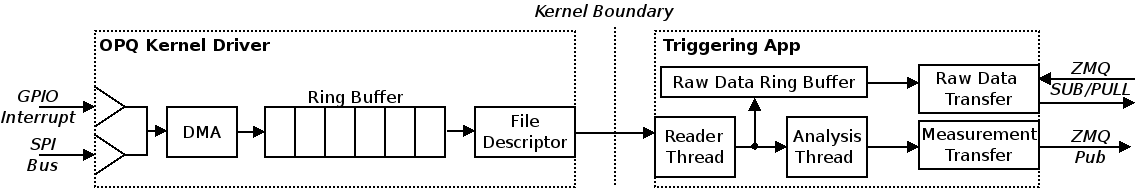
\includegraphics[width=0.9\textwidth]{images/opq-box/opqbox_software.png}
  \end{center}
  \caption{Block diagram of the OPQ Box 2 software stack.}
  \label{fig:opq:3}
\end{figure}

A Raspberry Pi single board computer (SBC) is responsible for signal analysis and anomaly detection.
The Raspberry Pi model used in OPQ Box is the Pi Zero W equipped with 256MB of main memory and a single core 1GHz ARM11 CPU. It also contains an on-board 802.11n WIFI transceiver, which removes the need for an external WIFI dongle.

\subsubsection{Software}\label{subsec:software}

The software stack of the Raspberry Pi aims to deliver an accurate and precise power quality analysis framework despite the rather limited capabilities of the hardware.
A block diagram of the software stack is shown in Figure~\ref{fig:opq:3}.
Digital data is transferred from the DSP to the Raspberry Pi via Serial Peripheral Interface, with the Pi acting as the master and the DSP as a slave device.
A hardware interrupt line is used to inform Pi software that the DSP is ready for the data transfer, and a kernel driver provides management of the SPI bus.
Internally, the OPQ driver maintains a ring buffer of 16 windows, each of which is 200 data samples in size.
Upon receiving the interrupt for the DSP, the CPU sets up the DMA transfer and the DMA engine transfers a 200 sample window into the kernel memory without CPU interaction.
This scheme requires the CPU to only service 60 interrupts a second, with each interrupt requiring on the order of 100 instructions, for a CPU utilization of less than $1\%$ in normal operation.
Userland applications communicate with the kernel driver using a file descriptor, where every $read$ system call yields 200 samples of raw waveform.
As a result, the smallest window that a userland application may process is a single AC cycle of the grid mains.

The userland component of the OPQ Box software is a multi-threaded extensible analysis framework called Triggering.
The reader thread is responsible for transferring and accumulating data from the kernel driver.
The smallest data buffer that the Triggering application processes at any given time is 10 grid cycles or 2k samples.
Once the cycles are transferred to the userland and timestamped, they are passed to the analysis thread for feature extraction, as well as to the Raw Data Ring Buffer (RDRB).
Since internally all data is addressed using shared pointers, during data duplication no copying is required.
RDRS is capable of buffering up to an hour of data before it is overwritten, resulting in the RDBS maximum size of 100MB.

The analysis thread of the Triggering application performs feature extraction of the raw data windows of 2000 samples.
Four metrics are extracted from the data stream: (1) Fundamental frequency, (2) RMS Voltage, (3) Total Harmonic Distortion, and (4) Transients. Let's briefly discuss how each of these are computed.

\subsubsection{Fundamental Frequency}\label{subsec:fundamental-frequency}

The fundamental frequency is calculated by computing the zero crossings of the AC waveform.
In order to improve the accuracy of the frequency calculation one must first filter out as much noise as possible.
Since our sampling rate is quite high (12kSps) and the fundamental frequency is quite low (60Hz), it is very computationally expensive to perform this filtering in a single step.
Instead, filtering is accomplished via a set of two low pass finite impulse response (FIR) filters.
First filter has a passband of 0-600Hz allowing us to downsample the waveform to 1200 samples per second.
Next filter has a passband of 0-100Hz allowing for further removal of high frequency noise.
Finally, zero crossings are extracted and used for the frequency calculation.
The zero crossings themselves were calculated by using linear interpolation between two points which bracket the time axis.

\subsubsection{Root Mean Square Voltage}\label{subsec:root-mean-square-voltage}

Root mean square voltage ($V_{rms}$) in electrical power is the equivalent value of DC voltage which would dissipate the same power in the resistive load. $V_{rms}$ is a convenient measure for detecting voltage sags and swells, since they result in nominally higher and lower computed value.

Similarly to the frequency calculation, OPQ Box uses a 10 cycle window for a single $V_{rms}$ calculation. Unlike the frequency calculation, the input is not filtered a priori.

\subsubsection{Total Harmonic Distortion}\label{subsec:thd}

The OPQ Box calculates total harmonic distortion (THD) using the industry standard methodology.
It should be noted that in the power quality domain THD is expressed as a percentage as opposed to $\frac{dB}{\sqrt{Hz}}$ as used in other disciplines.
Operationally, OPQ Box computes THD for 10 cycles of the fundamental frequency.
First an FFT transforms the real voltage samples into its frequency components.
Next, the square of the harmonic bins are accumulated and scaled by the magnitude of the fundamental power.

\subsubsection{Transient Detection}\label{subsec:transient-detection}

OPQ Box transient detection is performed via filtering out of the fundamental frequency via an FIR high pass pass filter with a cutoff frequency of $400Hz$ and searching for a maximum value in the remainder.

It should be noted that this transient detection method is susceptible to THD fluctuations, since any harmonic above $400Hz$ will remain in the filtered waveform.
However, since the THD information is transmitted along with the transient detection metric, they can be correlated in downstream transient detection.

\subsubsection{Network Communication}\label{subsec:network-communication}

The computed fundamental frequency and $V_{rms}$ are transmitted to the Makai service for aggregation.
Data transmission is handled using ZeroMq software stack with Curve25519 elliptic curve encryption.
Each device holds a unique private and public key, as well as the servers' public key, allowing both the Makai service and the OPQ Box to verify its peer.
Internally, metrics transmission uses ZeroMq's PUB/SUB protocol.
This protocol is a publish subscribe topology, with each message containing the topic and a payload.
Additionally, ZeroMq allows for multiple sub peers with subscriptions forwarded to the publisher automatically via a side channel.
This allows for the aggregation service to be spread across multiple nodes, with minimal network overhead.

If the aggregation service determines that an anomaly has occurred, it is able to request raw waveform from the OPQ Box RDRB via a separate ZeroMq pub sub channel.
If the RDRB buffer contains data for the requested temporal range, OPQ Box transmits the available data to the aggregation service via a push pull ZeroMq channel.
Protobuf message serialization is used to encode messages across the OPQ ecosystem.

In order to make a distributed measurement, all of the OPQ Boxes on the OPQ network need to maintain an accurate time reference.
Time synchronization across multiple OPQ Boxes is accomplished using the Network Time Protocol.
The expansion port of the OPQ Box supports a GPS receiver.
However, since GPS receivers require line of sight to the sky, it was not used for deployment.
NTP performance has been verified against GPS resulting in time error of $8ms\pm 5ms$ which is typical for NTP running over the Internet with a nearby NTP server.

\subsubsection{Manufacturing}

Currently, there is no mechanism for mass production of OPQ Boxes, but all of the plans are available under an Open Source license, so interested organizations with some basic hardware engineering skills can build their own boxes.

Complete specifications for the OPQ Box hardware, firmware, and software are available \cite{negrashov_opq_2020}. As of the time of writing, a single OPQ Box can be manufactured for approximately \$100 in parts. The cost drops significantly with scale, for example, 100 OPQ Boxes can be manufactured for a cost of approximately \$75 in parts per device.



\subsection{OPQ Makai}
\label{sec:opq-makai}

OPQ Box provides an inexpensive hardware device for collecting four important power quality measures with high fidelity, but realizing its potential requires an innovative approach involving two-way communication between OPQ Boxes and the OPQ cloud-based services. To see why, consider the IEEE 1159 standard for single location power quality monitoring \cite{unruh_ieee_2018}.  For transient monitoring, IEEE 1159 suggests a sampling rate of at least 7680 samples/second, up to 1 Megasample/second. This implies that if the cloud service requires the high fidelity data from all OPQ Boxes, it would incur a very large bandwidth cost. At 20 Ksamples/second with 16bit samples, a single OPQ Box will generate 300Kb/second of network bandwidth. Several thousand devices would easily saturate a 1 GB network link. In addition, collecting and recording all of the raw waveform data from residential power quality meters could lead to security and privacy issues.

Network bandwidth saturation is a common problem for distributed sensor networks, and a common solution is called "self-triggering".  In this approach, each monitoring device is configured with a threshold value for one or more measures of interest. When the threshold for a measure of interest is exceeded, then and only then is data sent over the network to cloud-based services for analysis.

The problem with the self-triggering approach is that grid-wide power quality events do not affect the entire grid in the same way. For example, due to the grid’s hierarchical structure, a voltage sag on one sub-circuit can manifest as a sag of a different magnitude or even a swell on another \cite{kahle_power_2015}. This may result in a situation where some of the monitoring devices will not consider a power quality anomaly as an event, because it did not surpass the metric threshold, and simply ignore it. From an analysis perspective, however, it can be useful to get raw data from all of the affected devices, not just the ones that were the affected to the point where the box was triggered. This additional information can be used to localize the disturbance, as well as better evaluate its impact.

Since sending all the data is infeasible, and since the self-triggering approach can potentially miss important forms of information, OPQ implements a novel, hybrid centralized/decentralized data acquisition scheme which involves two-way communication between the OPQ Boxes and a cloud service called OPQ Makai. In this scheme, OPQ Boxes use local processing resources to feature extract the incoming waveforms while storing them locally for an hour. Each OPQ Box sends its feature data to OPQ Makai once a second, which we called the "triggering stream". Feature data is very small, on the order of a few kilobytes, and so this approach allows the sensor network to scale to thousands of devices with acceptable network bandwidth requirements.  OPQ Makai processes the incoming triggering stream and looks for anomalies. If an anomaly is present in only a single device, it is highly probable that the cause is local and not grid-level. On the other hand, if the triggering stream shows an anomaly temporally collocated across multiple devices, the entire network or a subset of the network may be queried for raw waveform data for a temporal region which corresponds to the disturbance in the triggering stream.

Our pilot study, discussed in Section \ref{sec:pilot-study} will provide examples of the novel analysis capabilities made possible by OPQ Box and OPQ Makai communication. In general, here are the main advantages of our hybrid centralized/decentralized approach over traditional self-triggering and the ``naive" approach of sending all of the data:

{\em Bandwidth usage is minimized.} Instead of sending the entirety of raw data, only extracted features are sent. This results in a tiny fraction of the bandwidth requirement when compared to raw waveforms. Furthermore, the temporal window which encompasses a single feature can be adjusted in real time. Thus, as soon as an anomalous behavior is observed in a subset of sensors, this window can be adjusted for a finer grained feature extraction.

{\em Effects of latency are minimized.} In this case, "latency" refers to the time required for OPQ Makai to process the incoming feature stream and decide whether to request high fidelity data from one or more OPQ Boxes. Even at 1M samples/second at 16 bits of resolution, the memory requirement to store 5 minutes of raw waveform without compression are on the order of 512MB, which is well within the realm of inexpensive single board computers such as Raspberry PI. With compression specifically suited to the signal of interest, the memory requirement can be reduced even further. In the case of the OPQ sensor network, OPQ Makai has an hour to process feature data and request high fidelity data from OPQ Boxes. During our pilot study, OPQ Makai always responded within a second or two.

{\em Cloud processing requirements are reduced.} Since feature extraction is already performed at the device level, cloud computation requirements are reduced. With the advent of the Internet of Things, the computational capacity of edge devices is increasing.

{\em Subthreshold data acquisition can improve understanding of grid-local anomalies.} OPQ Makai makes the decision to acquire raw waveform from OPQ Boxes. This allows analysis of data from devices which were only mildly affected or even not affected at all by the disturbance. This creates new possibilities for investigation of disturbance propagation across the sensed area, as will be discussed in Section \ref{sec:pilot-study}.

{\em Temporal locality allows OPQ to provide improved insights into power quality anomalies over traditional triggering algorithms.} By exploiting the idea of temporal locality, it is possible to ascertain the geographical extent of an anomaly with only coarse features. This allows for a simple robust algorithm which may be deployed at the sink node for anomaly detection.

\subsubsection{Design}

OPQ Makai is a distributed extensible microservice framework responsible for receiving the triggering stream from the OPQ Boxes, locating anomalous temporal regions and requesting raw waveform for the anomalous time ranges. As shown in Figure \ref{fig:makai-design}, Makai consists of four major components: Acquisition Broker, Triggering Broker, Event Service and the Acquisition Service.

\begin{figure}
\center 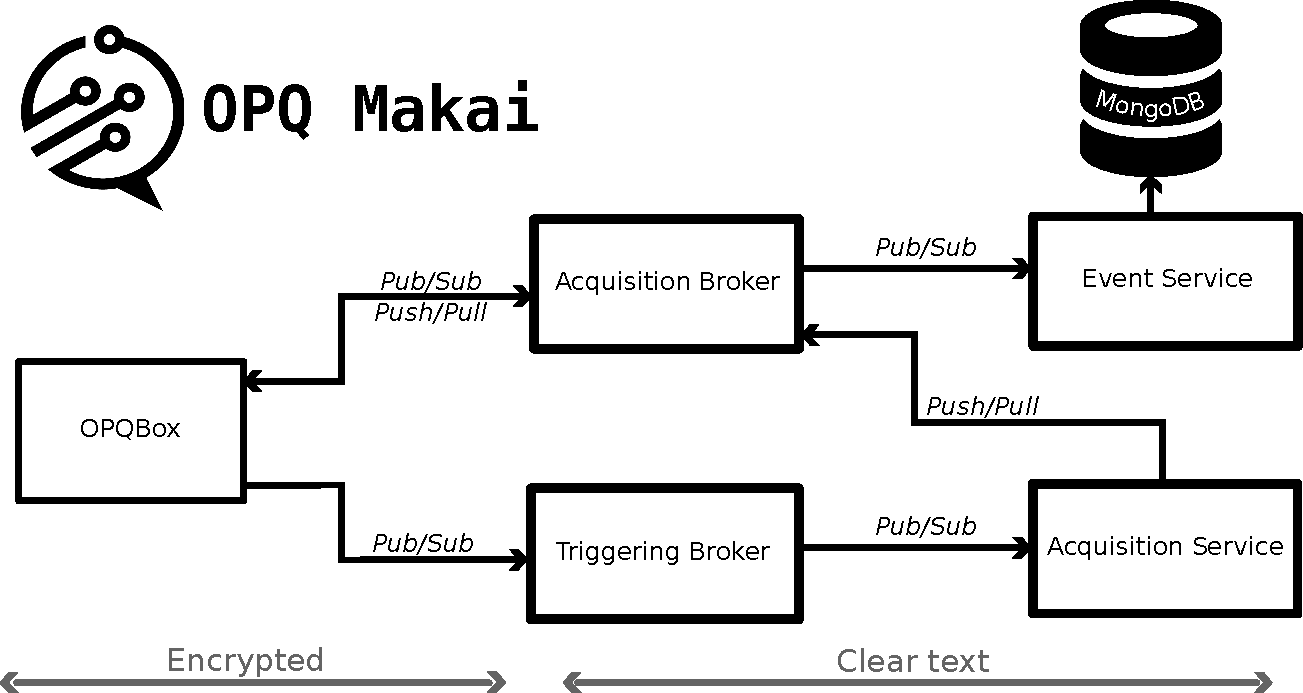
\includegraphics[width=3in]{images/makai/makai_main.pdf}
\caption{Makai component design}
\label{fig:makai-design}
\end{figure}

The Triggering Broker is perhaps the simplest component of the OPQ Makai system. The triggering stream generated by the OPQ Boxes is encrypted to preserve user privacy. In order to minimize the CPU time spent decrypting the data across multiple OPQ services, the Triggering Broker decrypts the data and sends clear text measurements to other OPQ cloud services. The Triggering Broker uses the ZeroMq subscribe socket to receive data from OPQ Boxes, and sends it via a publish socket to any connected client. Each publish message is published to a topic which corresponds to the ASCII representation of the originating OPQ Box ID. This allows services which utilize the Triggering Broker to select a subset of IDs to operate on. This is useful for load balancing the backend services, or dividing the OPQ network into separate regions with no electrical connections between them.

The Acquisition Broker manages the two-way communication between the OPQ Boxes and the rest of the cloud infrastructure. Unlike the triggering stream which originates from the OPQ Box, two-way communication is always initiated by OPQ cloud services. Two way communication is realized via a command response interface, where the OPQ service initiates the communication by sending a clear text command to the Acquisition Broker, which then forwards it in encrypted form to the appropriate OPQ Boxes.

The Acquisition Service resides between the Triggering and Acquisition Brokers. The Acquisition Service is responsible for three tasks:
(1) Computation of statistics of the incoming triggering stream; (2) Hosting plugins for triggering stream analysis; and (3) Generating data event requests for OPQ Boxes. The Acquisition Service accesses the triggering stream by connecting to the publish socket of the Triggering broker. Since the connection is managed through the ZeroMq publish-subscribe socket, several Acquisition Services can be connected to a single Triggering broker endpoint, each servicing a subset of OPQ Boxes by subscribing to only specific devices. The Acquisition Service does not include any analysis capabilities by default. Instead, analysis is performed by shared library loadable plugins. These plugins can be loaded and unloaded at runtime, thus allowing live upgrading and testing of new analysis methods.

The Event service is a microservice which stores raw data generated by OPQ Boxes in the MongoDB Database. On initialization, the Event service queries MongoDB database for the highest event number recorded so far, connects to the Acquisition Broker’s publish port, and subscribes to all messages that start with the prefix ``data”. This allows the Event service to capture every response from OPQ Boxes generated from commands issued by the Acquisition service plugins. Once the Event service receives a data response with an identity containing an event token it hasn’t seen before, it will increment the event number, and store it in an internal key value store.

\subsection{OPQ Mauka}
\label{sec:opq-mauka}

The previous sections discussed the design of OPQ Box, a custom hardware device for collecting four important measures of power quality, and OPQ Makai, a novel, hybrid centralized/decentralized data acquisition scheme which involves two-way communication between the OPQ Boxes.  As a result of these two innovations, an OPQ sensor network has the ability to collect and analyze high fidelity, low level data about power quality anomalies in a cost-effective, scalable fashion.

There are remaining challenges to creating a useful power quality sensor network. First, the data provided by OPQ Boxes is low-level, "primitive" data consisting of either features (i.e. frequency, voltage, THD, and transients) or waveform data. But what we actually want is actionable insights into grid stability. For example, we might want to know if a given anomalous data value is actually detrimental, or we might want to be able to predict when a power quality event might occur in the future based upon the recognition of cyclical events in the historical data.

A second challenge involves the potentially high volume of data might accumulate in the cloud. Although OPQ Box and OPQ Makai provide a scalable mechanism for communicating power quality data to the cloud services, it is still the case that, over time, a substantial amount of data could accumulate. One strategy is to simply store all of the data sent to the cloud forever. This means that data storage requirements will increase monotonically over time, making the sensor network more costly to maintain the longer it is in place. An alternative strategy is to implement an algorithm to identify uninteresting (or no longer interesting) data and discard it.  Ideally, such an algorithm would enable OPQ sensor network designers to calculate an upper bound on the total amount of cloud storage required as a function of the number of nodes (OPQ Boxes) in the network.

OPQ Mauka addresses both of these issues. First, OPQ Mauka provides a multi-layered representation for structuring and processing DSN data. The structure and processing at each layer is designed with the explicit goal of turning low-level data into actionable insights. Second, each layer in the framework implements a "time-to-live" (TTL) strategy for data within the level. This strategy states that data must either progress upwards through the layers towards more abstract, useful representations within a fixed time window, or else it can be discarded. The TTL strategy is useful because when implemented, it allows DSN designers to make reasonable predictions of the upper bounds on data storage at each level of the framework adjusting for the number of sensors and power anomaly probability.

 TTL also makes possible a ``graceful degradation" of system performance if those bounds turn out to be exceeded. For example, consider a situation in which a power network enters a prolonged period of widespread power quality instability, where every OPQ Box is reporting continuous anomalous conditions with respect to voltage, frequency, THD, and transients.  This ``worst case scenario" would lead to the potential situation of every OPQ Box trying to upload raw waveform data all the time. The TTL system provides safeguards, in that whatever low-level data has not been processed relatively quickly can be discarded.  Thus, instead of the system potentially going down entirely, it could instead continue to operate at a reduced capacity.

Figure \ref{fig:mauka-data-model} illustrates the hierarchical data model for OPQ Mauka. This data model can be conceptualized as a multi-level hierarchy that adaptively optimizes data storage using a tiered TTL approach and provides a mechanism in which typed aggregated data is continually refined to the point of being of becoming actionable. The data model also includes software components called "actors" that both move data upward through the levels and also apply optimizations downward through the levels. Actors are implemented through a plugin architecture, making it easy to experiment with the data model and improve it over time.

\begin{figure}
\center 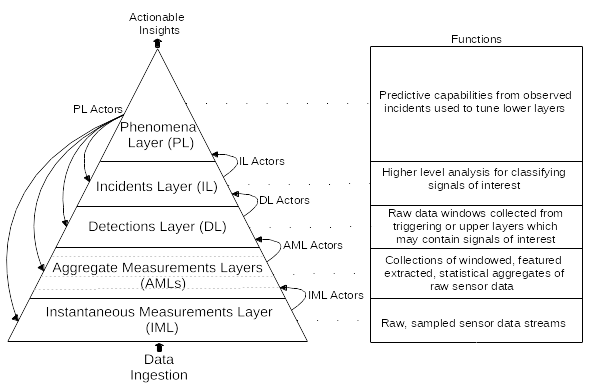
\includegraphics[width=4in]{images/mauka/mauka-data-model.png}
\caption{Mauka data model hierarchy}
\label{fig:mauka-data-model}
\end{figure}

The lowest layer of the hierarchy is the Instantaneous Measurements Layer (IML). The IML contains "raw" data, in other words, the digitized waveform.  IML data exists both on each OPQ Box (where it is available for up to the previous 60 minutes). It also exists in the cloud, in the event that OPQ's triggering mechanism has caused a temporal interval of waveform data to be uploaded. IML data in the cloud has a TTL of 15 minutes: unless the waveform data is found to be useful by a cloud service within 15 minutes, it can be discarded.

The second layer is the Aggregate Measurements Level (AML). The AML stores power quality summary statistics sent either once per second or once per minute by each OPQ Box. These summary statistics include the maximum, minimum, and average values of voltage, frequency, THD, and transient metrics over the time window. It is AML data that is used to initiate the triggering process of uploading IML data from the cloud.

The third layer is the Detections Level (DL). This layer is responsible for processing the IML and AML data to produce a representation of an "event" with a precisely defined start and end time based upon examination of the waveform.  As will be discussed in Section \ref{sec:subthreshold-events}, knowledge of the start and end time of a power quality anomaly allows investigation of how that anomaly might manifest itself elsewhere in the grid, even if this manifestation is not severe enough to produce over-threshold data values.

The fourth layer is the Incident Level (IL).  This layer starts to answer the question of whether the data is "actionable" by classifying the detected event according to various industry standards for power quality anomalies: IEEE 1159, ITIC, SEMI F47, and so forth.  For example, an event that falls into the ITIC "prohibited" region clearly indicates a power quality anomaly that requires further study and intervention.

The fifth and final level is the Phenomena Level (PL). This layer contains the results of analyses that attempt to identify cyclic, and thus predictable, power quality disturbances. It also contains analysis results regarding the similarity of various incidents, which can help uncover causal factors.  Finally, it provides analyses for adaptive optimization of the OPQ Sensor Network. These optimizations can change the thresholds for individual boxes to either increase their sensitivity or decrease their sensitivity over specific intervals of time. The ultimate goal of adaptive optimization is to help the network learn to acquire all of the data useful for analyses, and only the data useful for analyses.  We are still in the early stages of exploring the potential of adaptive optimization in OPQ networks.

\subsubsection{OPQ Mauka Actors}

The current capabilities of OPQ Mauka can be summarized in terms of its Actors, which are implemented as plugins. Nine of the most important Actors are described below.

{\em Makai Event Actor.} The Makai Event Actor is responsible for reading data newly created by OPQ Makai into OPQ Mauka. It performs feature extraction on the raw data stream and forwards those features (or the raw data) to subscribing Actor plugins. This allows OPQ Mauka to perform feature extraction once, and allow use of those features by multiple Actors.

{\em Frequency Variation Actor.} The Frequency Variation Actor classifies generic frequency sags, swells, and interruptions as defined by the IEEE 1159 standard. Both duration and deviation from nominal are used to perform these classifications. Duration classifications include frequency deviations that last for less than 50 ns, between 50 ns to 1 ms, and 1 ms to 50 ms. Classifications for deviations from nominal are performed for values that are up to 40\% deviation from nominal. This Actor is able to classify frequency swells, frequency interruptions, and frequency sags, leading to the creation of data at the Incident Layer.

{\em IEEE 1159 Voltage Actor.} The IEEE 1159 Voltage Actor is used to classify voltage Incidents in accordance with the IEEE 1159 standard[29]. In general, this standard classifies voltage disturbances by duration and by magnitude. Voltage durations are classified from 0.5 to 30 cycles, 30 cycles to 3 seconds, 3 seconds to a minute, and greater than 1 minute. Voltage deviations are classified in both the sag and swell directions as a percentage from nominal. Sags are generally classified between 10\% and 90\% of nominal while swells are generally classified from 110\% to 180\% of nominal. This Actor is capable of classifying voltage sags, swells, and interruptions as defined by the standard, and creating data at the Incident Layer if appropriate.

{\em Box Optimization Actor.} The Box Optimization Actor is responsible for sending and receiving typed messages to and from OPQ Boxes from OPQ Mauka. This Actor is capable of requesting the state of each OPQ Box (e.g. uptime, Measurement rate, security keys, etc). It is also capable of adjusting the state of individual OPQ Boxes by changing things such as the Measurement and Trend rate or the sampling rate used by the Box.

{\em Future Phenomena Actor.} The Future Phenomena Actor is responsible for creating Future or Predictive Phenomena. These Phenomena are used to predict Events and Incidents that may occur in the future. This plugin does not subscribe to any messages, but instead utilizes timers to perform its work. By default, this plugin runs every 10 minutes.

When a Future Phenomena Actor runs, it loads any active Periodic Phenomena found in the database. If Periodic Phenomena are found, this Actor extrapolates possible Detection and Incident Layer data by first examining their timestamps and then extrapolating into the future using the mean period and the standard deviation. For each timestamp in a Periodic Phenomena, the mean period is added. If the resulting timestamp is in the future, a Future Phenomena is created using the time range of the future timestamp plus or minus the standard deviation of the Periodic Phenomena.

When a Future Phenomena is created, timers are started in a separate thread signifying the start and end timestamps of the Future Phenomena. When the first timer runs, messages are sent to the Box Optimization Actor and the Threshold Optimization Actor instructing OPQ Box thresholds to be set lower and measurement rates to be set higher. This increases the chance of seeing an anomaly over the predicted time window. When the second timer runs, these values are reset to their default values. Thus, the plugin increases fidelity and decreases thresholds over the period of a Future Phenomena.

{\em ITIC Actor.} The ITIC Actor analyzes voltage to determine where it falls within the ITIC curve \cite{thallam_power_2000}. The ITIC curve is a power acceptability curve that plots time on the x-axis and voltage on the y-axis.  The purpose of the curve is to provide a tolerance envelope for single-phase 120V equipment. The curve defines three regions. The first region is "No Interruption" and generally includes all voltages with very short sustained durations. All events within this region have no noticeable effect on power equipment. The second region, the "No Damage Region", occurs during voltage sags for extended periods of time. Power Events in this region may cause equipment interruptions, but it will not damage the equipment. The final region, the "Prohibited" region, is caused by sustained voltage swells and may cause damage to power equipment. This Actor determines if an event falls within the "No Damage" or "Prohibited" regions and if so, creates an Incident to record this.

{\em SEMI F47 Actor.} The SEMI F47 Actor is similar to the ITIC Actor in that it plots voltage and duration against a power acceptability curve. In this case, the standard used is the SEMI F47 standard \cite{djokic_sensitivity_2005}. Rather than using a point-in-polygon approach, this plugin reads the voltage features sequentially and uses a state machine to keep track of the current classification. This plugin only classifies values as a "violation" or as "nominal".

{\em Transient Actor.} The Transient Actor is responsible for classifying frequency transients in power waveforms. The plugin subscribes to messages from a topic which contains a calibrated power waveform payload. The Transient Actor is capable of classifying impulsive, arcing, oscillatory, and periodic notching transients. A decision tree is utilized to select the most likely transient type and then further analysis is used to perform the actual classification of transients. Dickens et al \cite{dickens_transient_2019} provides more details on the transient classification system used by this Actor.

{\em Periodicity Actor.} The Periodicity Actor is responsible for detecting periodic signals in power data. This Actor does not subscribe to any messages, but instead runs off of a configurable timer. The Actor is set to run by default once an hour and every hour it scrapes the last 24 hours worth of data and attempts to find periods in the Measurements over that duration.

For each feature in the Measurement and Trend data (e.g. frequency, voltage, and THD), the Periodicity Actor first removes the DC offset from the data by subtracting the mean. Next, the Actor filters the signal using a 4th order high-pass filter to filter out noise. The Actor then performs autocorrelation on the signal followed by finding the peaks of the autocorrelation. The mean distance between the peaks of the autocorrelation provides the period of the signal.

The Periodicity Actor only classifies data as periodic if at least 3 peaks were found and the standard deviation of the period is less than 600 seconds (10 minutes). Once a positive identification has been made, peak detection is performed on the original signal. Once the plugin has the timestamps and deviations from nominal of the periodic signal of interest, the plugin can group Measurements, Trends, Detection Layer Events, and Incidents that were created during the periodic signals together as part of the Periodic Phenomena.

\subsection{OPQ View}
\label{sec:opq-view}

The final component of the OPQ Sensor Network system architecture is called OPQ View. It is a web application, implemented using the Meteor application framework, which provides a variety of visualization and query services.  An example of the OPQ View home page is provided in Figure \ref{fig:opq-view-home}.

\begin{figure}
\center 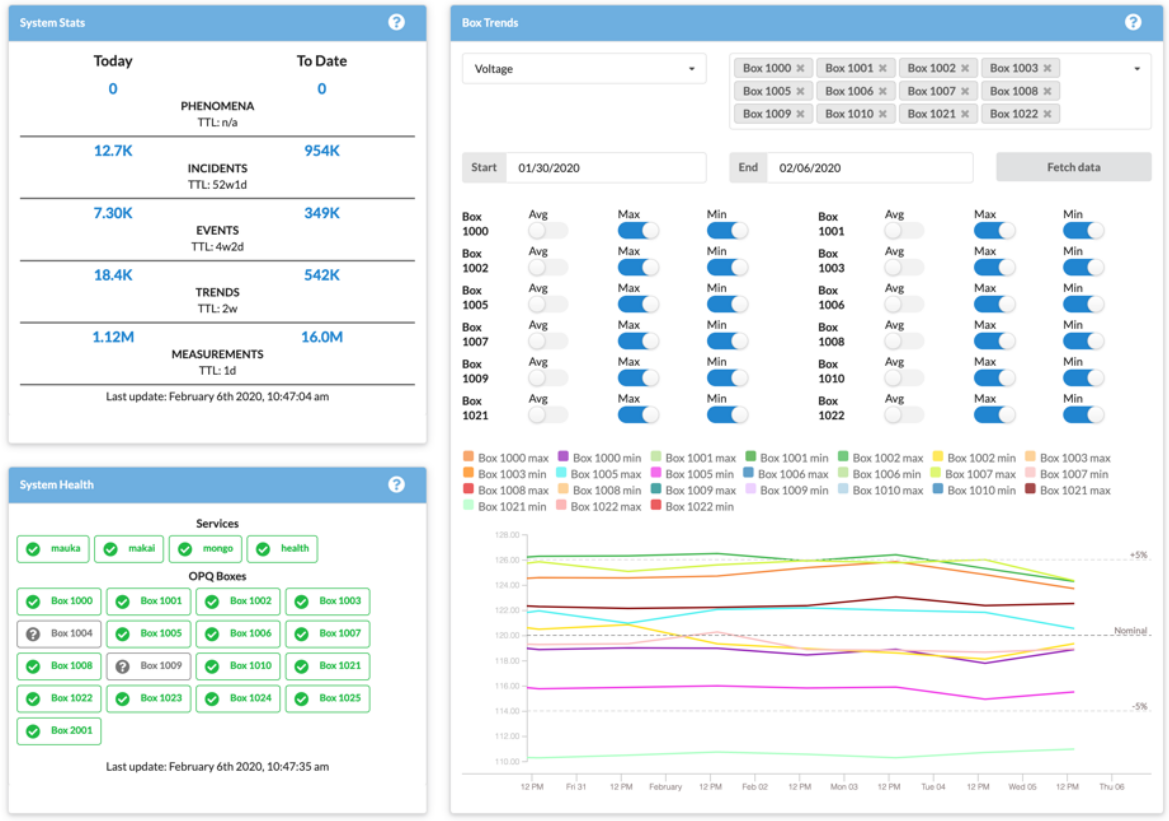
\includegraphics[width=5in]{images/view/homepage.png}
\caption{OPQ View: home page}
\label{fig:opq-view-home}
\end{figure}

The home page provides three components:  a "System Stats" window which indicates the number of data elements currently at each level of the OPQ Mauka data hierarchy, a "System Health" window that indicates whether the Cloud services appear to be running correctly and the status of communication with all known OPQ Boxes on the sensor network, and a "Box Trends" visualization that provides the ability to quickly see trends in the four basic measures (Voltage, Frequency, THD, and Transients) over time.

Figure \ref{fig:opq-view-box-map} shows a map-based view of the sensor network. This figure shows the location of 11 OPQ Boxes on the University of Hawaii campus at one point during Fall of 2019. Depending on the zoom level of the interface, some boxes are collapsed into disks with a number indicating the number of boxes at that location. Zooming in reveals more information about the box including near-real time values for voltage and frequency, as is shown for the box in the upper right corner of the figure.

\begin{figure}
\center 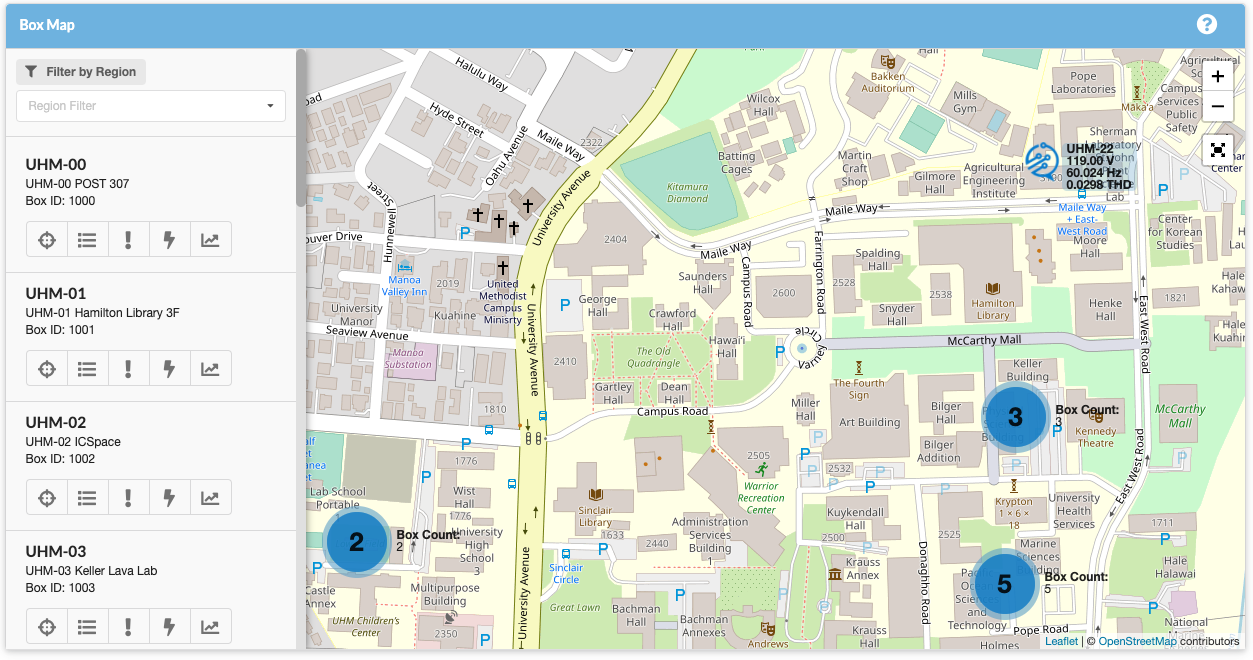
\includegraphics[width=5in]{images/view/boxmap-2.png}
\caption{OPQ View: Box Map}
\label{fig:opq-view-box-map}
\end{figure}

Figure \ref{fig:opq-view-incident-summary} shows a visual display of a single Incident. This view includes a map-based location of the box whose data was involved in the Incident, the start and end time and duration of the Incident, the classification(s) of the anomalous data, and the waveform associated with the Incident (when applicable). If additional analysis is desired, the raw data can be downloaded in CSV format.

\begin{figure}
\center 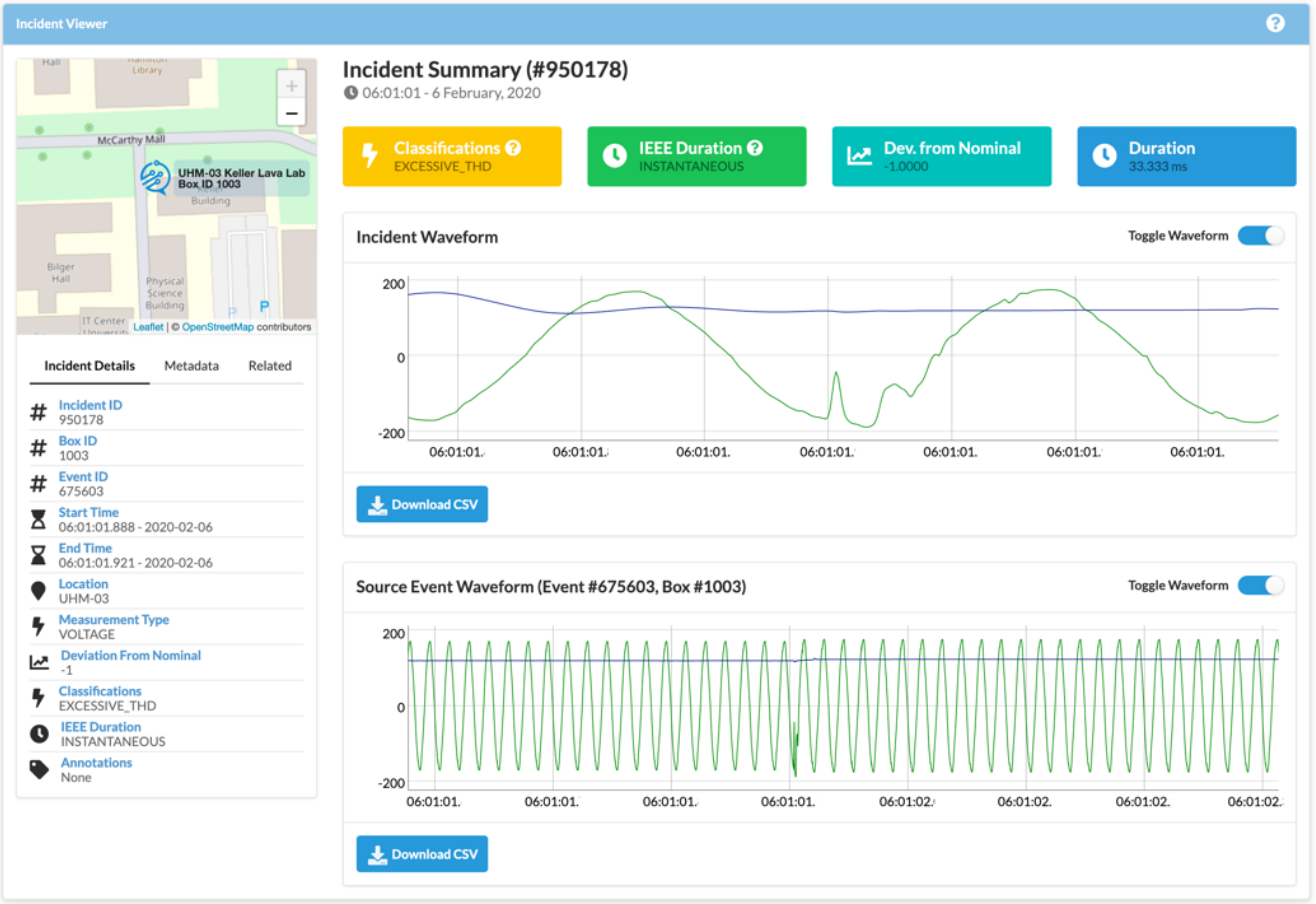
\includegraphics[width=5in]{images/view/incident-summary.png}
\caption{OPQ View: Incident Summary}
\label{fig:opq-view-incident-summary}
\end{figure}

The above images provide a sense for how OPQ View helps users to understand, monitor, and assess an OPQ Sensor Network and the underlying power quality of the grid it is attached to. There are several features in OPQ View for user and box management; for details, please see the OPQ View documentation.

While OPQ View provides a variety of useful visualization and analysis features, users wishing to understand the power quality of their grid are not restricted to its current feature set. The OPQ database schema is public, and if a new analysis is desired, it is straightforward to query the database directly for the data of interest and build a new analysis off of it.


















